\chapter{Aufbau und Konfiguration des Clusters}

Dieses Kapitel bildet die erste Hälfte des praktischen Teils der Projektarbeit.
Dieser behandelt den Aufbau der Hardware, die Netzwerk Konfiguration, sowie die Installation der Kata-Runtime und letztendlich den Aufbau eines Kubernetes Clusters.
Am Ende diese Kapitels soll alles für das sichere Deployment von Sormas auf Kata Vorbereitet sein.  

\section{Hardware}
Für das Projekt wurde folgende Hardware verwendet:
\begin{itemize}
    \item 1 Intel Atom \ac{NUC}
    \item 3 Lenovo Workstations 
    \item 1 Linksys Netzwerk-Switch
    \item 5 Ethernet Kabel
    \item 1 \ac{PDU}
    \item entsprechende \ac{PSU}s
\end{itemize}

Der einzelne Intel \ac{NUC} soll in dem Cluster die Rolle des Masters einnehmen.
Die Workstations werden als Worker eingesetzt.
Der Switch und die Ethernet Kabel werden genutzt um ein isoliertes Netzwerk aufzubauen, davon wird sich eine geringere Latenz und bessere Labor Bedingungen versprochen.
Mithilfe der \ac{PDU} und \ac{PSU}s wird das Cluster mit Strom versorgt. 
Eine Bestimmung der Hardware lässt sich Tabelle \ref{table:hardware} entnehmen, für eine detallierte Version siehe Anhang \ref{table:hw_detail}.

\begin{table}[h]
    \centering
    \begin{tabular}{ p{ 0.3\textwidth } | p{ 0.3\textwidth } p{ 0.3\textwidth } }
        x & \ac{NUC} & Workstations \\
        \hline \\
        CPU & Intel\textregistered Celeron\textregistered N2930 CPU@1.83GHz &  Intel\textregistered Core\texttrademark i3-7100 CPU@3.90GHz \\
        Cores & 4 & 4 \\
        Arbeitsspeicher & 8GB & 8GB \\
        Speicherplatz & 196GB & 240 GB \\
    \end{tabular}
    \caption{Hardware}
    \label{table:hardware}
\end{table}


\section{Vorbereitung der Maschinen}
Um die Maschinen vorzubereiten wurden bei jeder einzelnen der Storage komplett formatiert.
Anschließend wurde auf allen Maschinen Ubuntu 20.04 als \ac{OS} installiert.
Ubuntu wurde auf Empfehlungen aus dem Unternehmen gewählt, da einige schon gute Erfahrungen mit Kubernetes auf Ubuntu gesammelt haben und ein gutes Tiefewissen vorhaben ist.
\\
Für jede Maschine wurde dabei ein User und ein Passwort eingerichtet, sowie der \ac{SSH} Zugriff von Außerhalb freigeschaltet.
Der SSH-Zugriff wird benötigt um die Maschinen leichter zugänglich zu machen, aber vor allem, um Sie mit Ansibel managen zu können.


\section{Netzwerk Konfiguration}
Als nächstes muss ein Netzwerk-Zugang für die Maschinen eingerichtet werden.
Das Netzwerk soll so gut wie möglich von den Produktiv-Netzwerken bei Netzlink abgegrenzt sein.
Durch ein Subnet kann erreicht werden, dass die Netzwerk Performance erhöht wird und die Maschinen nicht von anderem Traffic beeinflusst werden können.
Dadurch können insgesamt reproduzierbarere Ergebnisse erzielt werden. 
\\
Für diese Projekt soll des Subnetz von dem Master-Node aufgespannt werden. 
Dadurch kann der Master auch an anderer Stelle einfach mit dem Netzwerk verbunden werden und das interne Netz bleibt unverändert.
Für den Master wurde also eine statische Netzlink-Interne \ac{IP}-Adresse angefragt um über diese Adresse auch die restlichen Nodes an das Netzwerk anzuschließen.
Zusätzlich erhält der Master eine interne \ac{IP}-Adresse über die er mit den Nodes kommunizieren kann.
Die gewählten Adressen lassen sich Tabelle \ref{table:katanetes_ips} entnehmmen.

\begin{table}
    \centering
    \begin{tabular}[h!]{ c | c c }
        x & Externe \ac{IP} & Interne \ac{IP} \\
        \hline
        k8smaster & 10.10.6.60 & 192.168.0.1 \\
        k8sworker1 & - & 192.168.0.11 \\
        k8sworker2 & - & 192.168.0.12 \\
        k8sworker3 & - & 192.168.0.13 \\
    \end{tabular}
    \caption{Cluster IPs}
    \label{table:katanetes_ips}
\end{table}

Das Netzwerk wurde so geplant, dass nur der Master-Node einen Internet-Zugriff beötigt.
Auf Ihm wurde ein \ac{DHCP}-Daemon so eingerichtet, dass dieser jedem der Worker basierend auf deren \ac{MAC}-Addressen die richtige IP zuordnet. 
Die Configuration für den \ac{DHCP}-Server findet sich im Anhang unter \ref{app:dhcp}. 

Um den Maschinen den Internet-Zugang zu ermöglichen muss als letztes \ac{NAT} auf dem Master Node konfiguriert werden.
Dafür muss \textbf{net.ipv4.ip\_forward=1} in die \textit{/etc/sysctl.conf} eingetragen werden und anschließend der Server rebootet.
Außerdem müssen die \textbf{iptables} Regeln angepasst werden, damit der Traffic auf dem internen Interface auf das externe Interface weitergeleitet wird. 
Das externe Interface ist das \textbf{enp4s0} und das Interne ist \textbf{enp3s0}.
Für das externe Interface, also \textbf{enp4s0} muss zunächst \textbf{POSTROUTING} und \textbf{MASQUERADE} eingerichtet werden. 
Dadurch werden die Pakete, die an diesem Interface ankommen, mit der IP des Masters maskiert und dann surch das public Interface gesendet. 

Anschließend müssen alle Pakete die an \textbf{enp3s0} geschickt werden auf \textbf{enp4s0} geforwarded werden, sowie die ankommenden Pakete auf \textbf{enp4s0} wieder über \textbf{enp3s0} zu den entsprechenden Maschienen.

Die genau Konfiguration ist im Anhang unter \ref{app:iptables} zu finden. 

In Ubuntu 20.04 wird nicht wie vielleicht bekannt mit der rc.local gearbietet, sondern mit den Tools \textbf{iptables-persistent} und \textbf{iptables-save}.

Das entstandene Netzwerk wird in Abbildung \ref{fig:network_diagramm} dargestellt.

\begin{figure}[h]
    \centering
    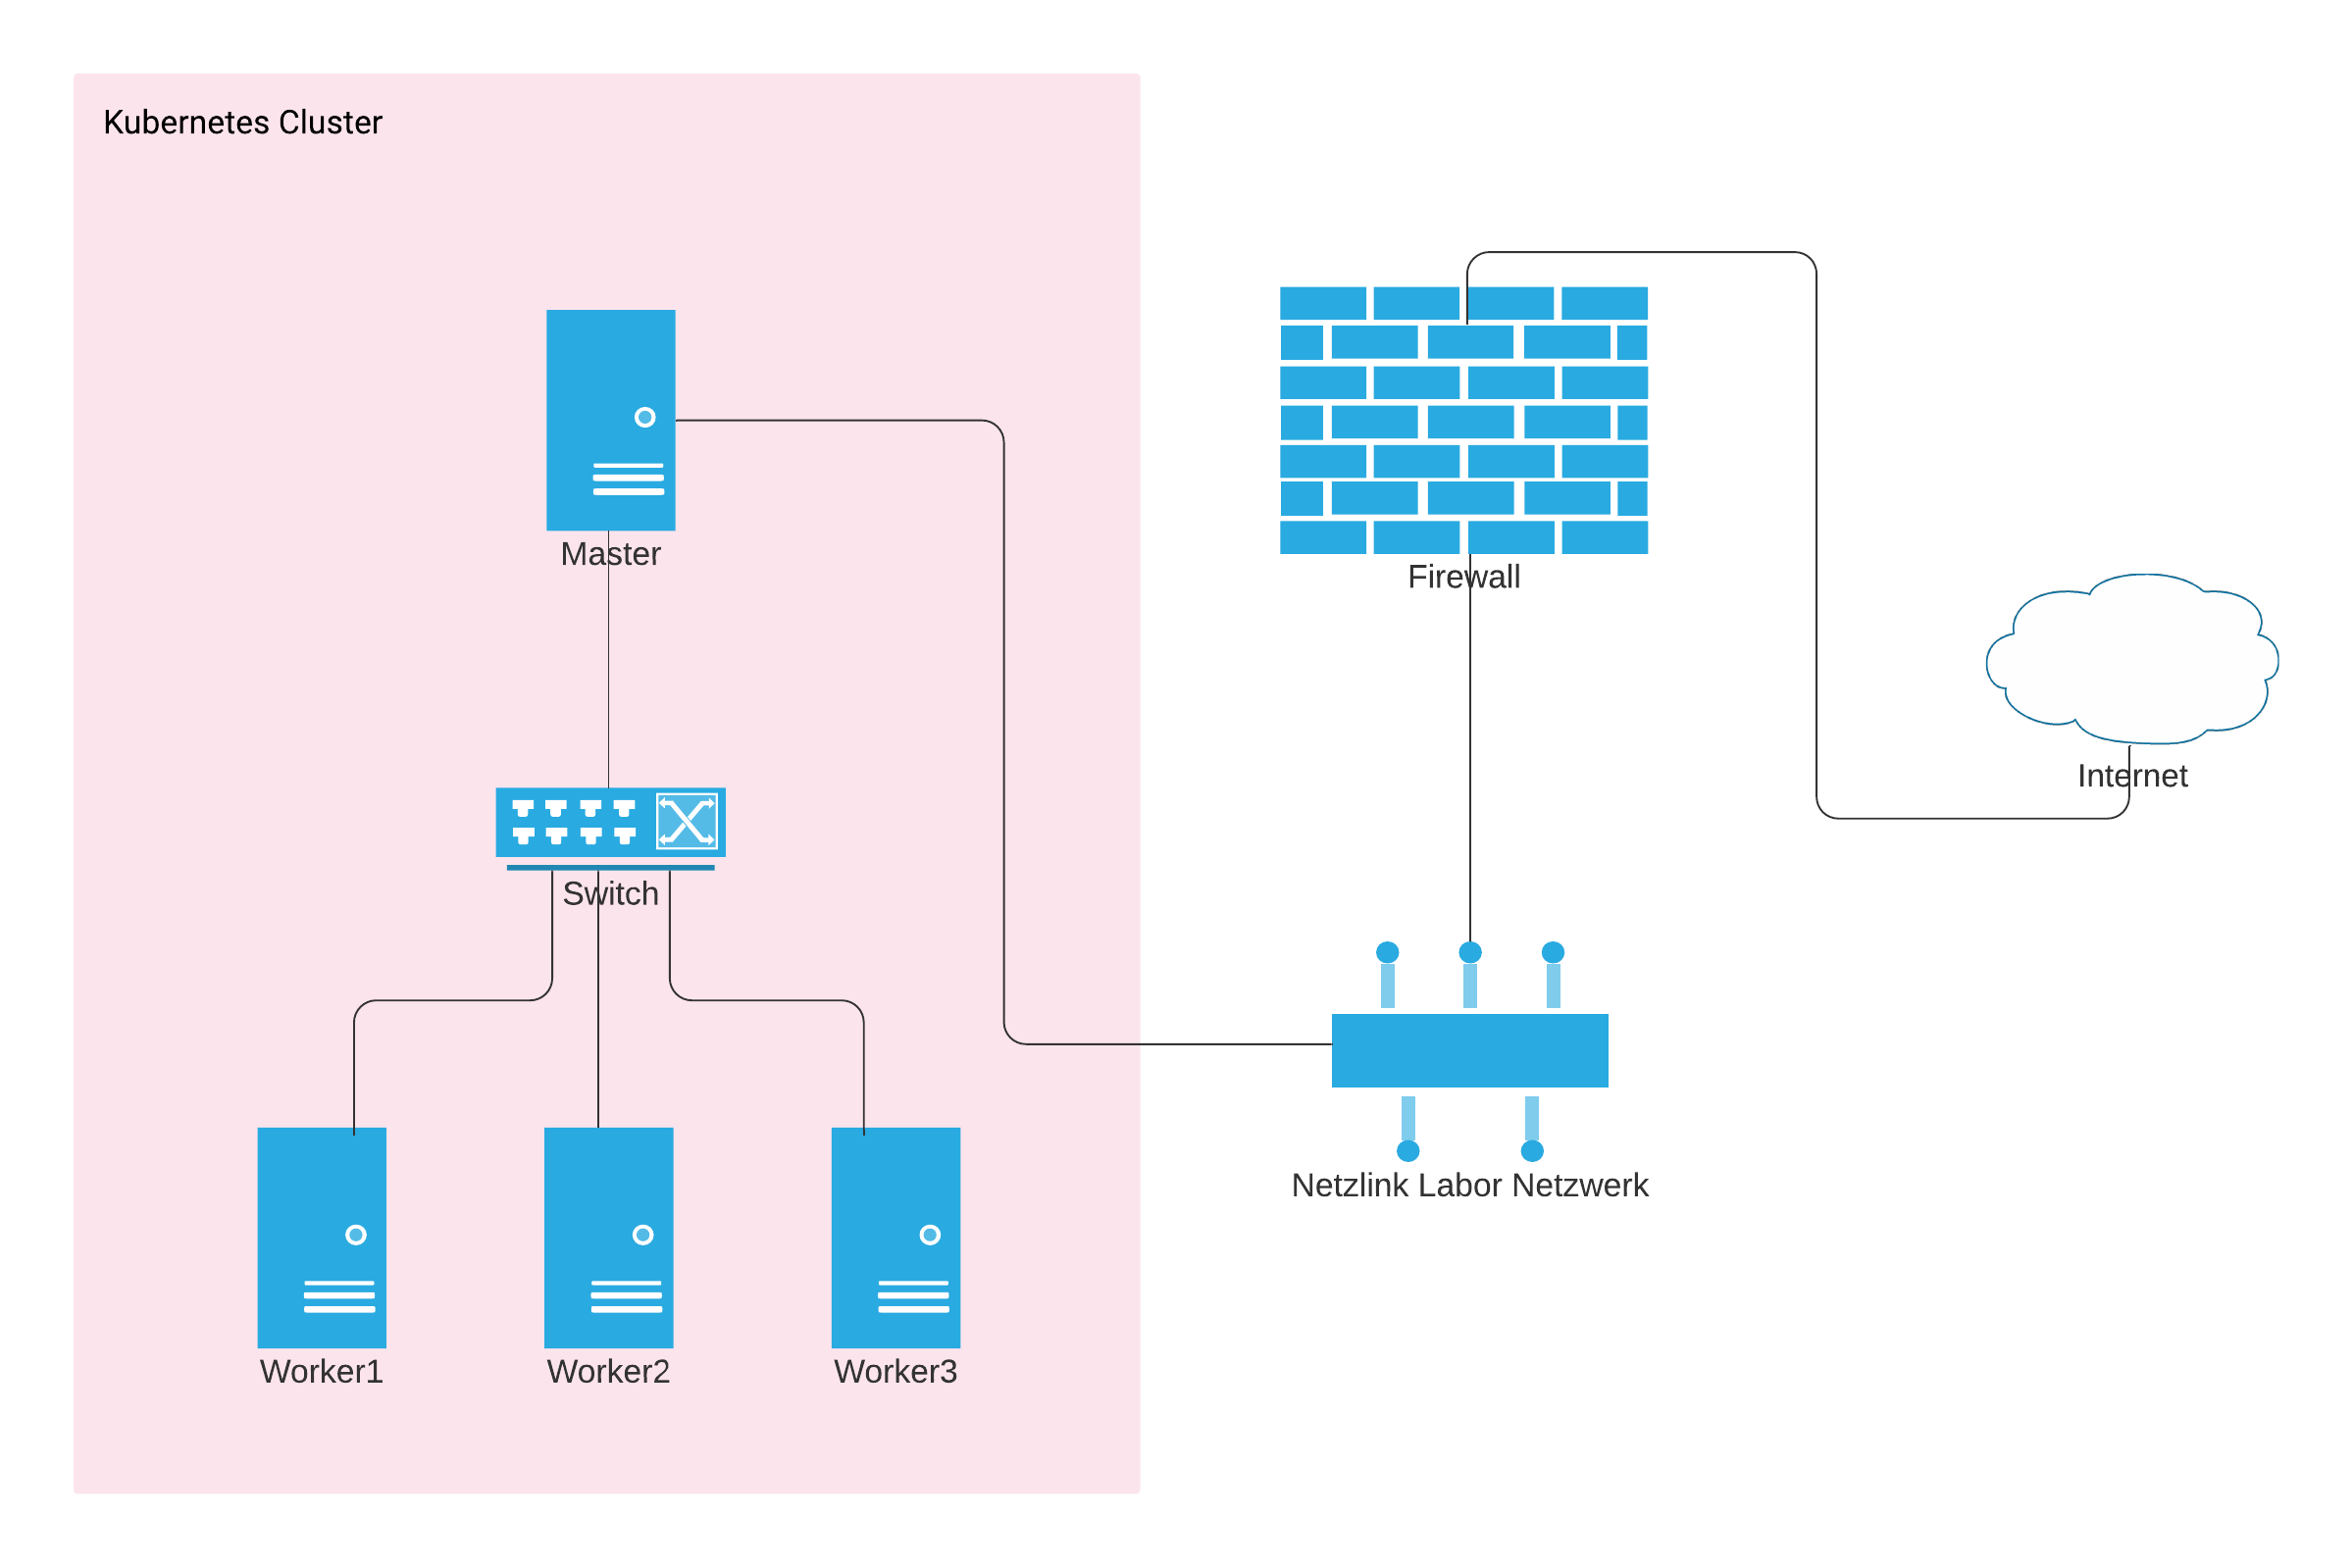
\includegraphics[width=\textwidth]{bilder/Katanetes Network.png}
    \caption{Netzwerkdiagramm}
    \label{fig:network_diagramm}
\end{figure}

\newpage

\section{Ansible Setup}
Von diesem Punkt an können nun alle Konfigurationen mit Ansible gemacht werden, da auf jeder der Maschinen \ac{SSH} konfiguriert ist und sie alle über eine Netzwerkverbindung verfügen.
Dazu muss nur auf dem Master Ansible installiert werden und der \ac{SSH} Zugang zu allen Zielsystemen konfiguriert sein. 
Für die Installation von Ansibel muss zunächst das Repository \textbf{ppa:ansible/ansible} zum Paketmanager hinzugefügt werden, dann können über \textbf{apt} die entsprechenden Pakete installiert werden.
Wie zuvor erwähnt muss die Ansibel Installation nur auf einer Maschine erfolgen.

Anschließend müssen für Ansible nur die Hosts, welche gemanaged werden sollem, in die \textit{hosts}-file eingetragen werden.
Dabei bietet Ansible die Möglichkeit Hostgruppen zu bilden. 
Wenn ein Playbok ausgeführt wird, kann die Hostgruppe angegeben werden, und alle Operationen werden dementsprechend auf alle Hosts in dieser Gruppe angewendet. 
Für dieses Projekt wurden die Gruppen \textbf{master} und \textbf{woker} gebildet.
Das Inventory kann im Anhang unter \ref{app:hosts_file} gefunden werden.

\section{Installation und Konfiguration von Kata}

Damit Kubernetes mit Kata-Containern als Runtime aufgebaut werden kann, muss die Runtime als erstes installiert werden.
Kata benötigt eine \ac{KVM}-Software um zu funktionieren, hier wurde qemu-kvm gewählt.
Pakete die im Paket-Manger des \ac{OS} enthalten sind, können mittels des entsprechenden Ansible-Moduls installiert werden.
Für Ubuntu ist dies das \textbf{apt} Modul. 

Zur Installation von Kata wird das Tool \textbf{kata-manager}\footnote{https://github.com/kata-containers/documentation/blob/master/install/installing-with-kata-manager.md} angeboten. 
Dieses hat zwei verschiedene Installations Modi:
\begin{itemize}
    \item Full Installation \\ Hier werden die Kata-Pakete installiert, dann Docker und zuletzt wird Docker konfiguriert um standartmäßig die Kata-Runtime zu nutzen
    \item Kata packages \\ Hier werden ausschließlich die Kata-Pakete installiert
\end{itemize}
Da Kuberntes mit Containerd Installiert werden soll, wird hier auf eine zusätzliche Docker Installation verzichtet.
Um den Kata-Manager auszuführen kann einfach das Skript mit \textbf{curl} heruntergeladen werden und dann in einer Shell ausgeführt:
\begin{lstlisting}[language=bash]
    $ bash -c "$(curl -fsSL https://raw.githubusercontent.com/kata-containers/tests/master/cmd/kata-manager/kata-manager.sh) install-packages"
\end{lstlisting}




\section{Installation des Kubernetes-Clusters}

